\section{流水线并行：按深度切分}

流水线并行的思路是：\textbf{模型太深时，把层切到不同 rank 上。} 这样每个 rank 只负责一段层堆栈，前一个 rank 算完就把激活传给下一个 rank。

\begin{figure}[H]
\centering
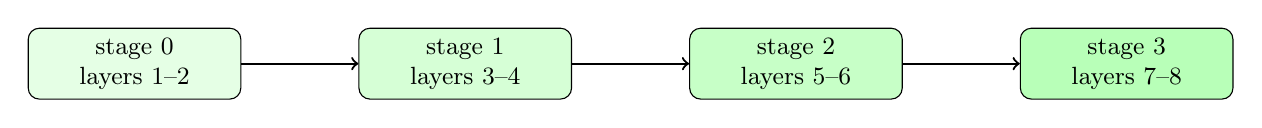
\begin{tikzpicture}[every node/.style={font=\small, align=center}]
\node[draw, rounded corners, fill=green!10, minimum width=2.7cm, minimum height=0.9cm] (s0) at (0,0) {stage 0\\layers 1--2};
\node[draw, rounded corners, fill=green!16, minimum width=2.7cm, minimum height=0.9cm] (s1) at (4.2,0) {stage 1\\layers 3--4};
\node[draw, rounded corners, fill=green!22, minimum width=2.7cm, minimum height=0.9cm] (s2) at (8.4,0) {stage 2\\layers 5--6};
\node[draw, rounded corners, fill=green!28, minimum width=2.7cm, minimum height=0.9cm] (s3) at (12.6,0) {stage 3\\layers 7--8};
\draw[->, thick] (s0) -- (s1);
\draw[->, thick] (s1) -- (s2);
\draw[->, thick] (s2) -- (s3);
\end{tikzpicture}
\caption{流水线并行的切分方式：层分到不同 stage，激活在 stage 之间流动}
\end{figure}

\subsection{为什么要 microbatch}

如果一个大 batch 整体往前推进，后面的 stage 会空等前面的 stage。这种空闲就是 pipeline bubble。解决方法是把 batch 切成 microbatches，让不同 stage 同时处理不同 microbatch，从而提高利用率。

\begin{figure}[H]
\centering
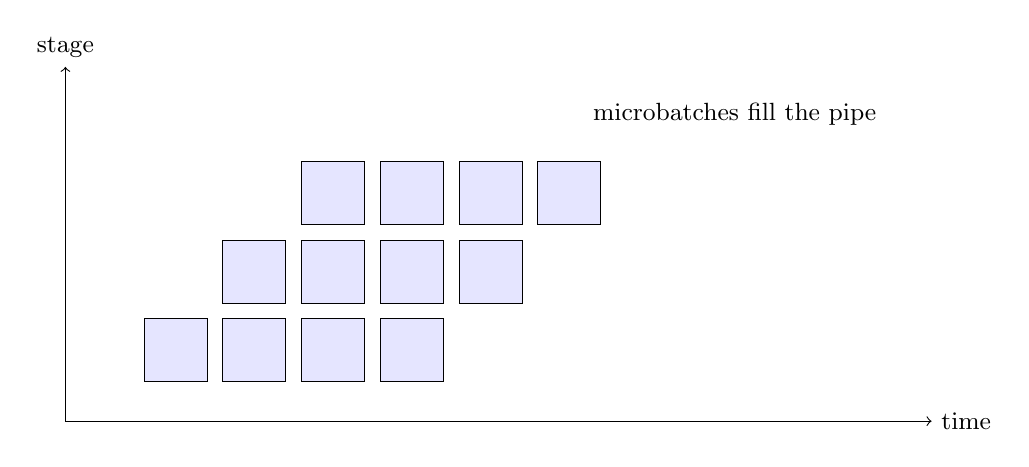
\begin{tikzpicture}[every node/.style={font=\small}]
\draw[->] (0,0) -- (11,0) node[right]{time};
\draw[->] (0,0) -- (0,4.5) node[above]{stage};
\foreach \x in {1,2,3,4}{
    \draw[fill=blue!10] (\x,0.5) rectangle ++(0.8,0.8);
    \draw[fill=blue!10] (\x+1,1.5) rectangle ++(0.8,0.8);
    \draw[fill=blue!10] (\x+2,2.5) rectangle ++(0.8,0.8);
}
\node at (8.5,3.9) {microbatches fill the pipe};
\end{tikzpicture}
\caption{microbatch 让流水线不再空转}
\end{figure}

\begin{knowledgebox}{bubble 的直觉}
stage 越多，启动和收尾的空档越明显。microbatch 越少，空档越浪费；microbatch 越多，利用率越高，但调度也更复杂。
\end{knowledgebox}

\subsection{流水线为什么总有空档}

流水线并行的难点不是“能不能传过去”，而是“什么时候能持续传”。当最前面的 stage 刚开始工作时，后面的 stage 还没拿到激活；当最后的 stage 已经快结束时，前面的 stage 也没法继续喂新数据。这种首尾空档是流水线天然会有的。

\begin{importantbox}{microbatch 的作用}
microbatch 本质上是在增加流水线里的“在途任务数”。在途任务越多，stage 的空转越少；但 microbatch 太碎又会增加调度次数和通信次数，所以这里也不是越多越好。
\end{importantbox}

\begin{figure}[H]
\centering
\begin{tikzpicture}[every node/.style={font=\small, align=center}]
\node[draw, rounded corners, fill=green!10, minimum width=3.5cm, minimum height=0.9cm] (u1) at (0,0) {前几步\\fill pipeline};
\node[draw, rounded corners, fill=green!18, minimum width=3.5cm, minimum height=0.9cm] (u2) at (4.8,0) {中间阶段\\稳定流动};
\node[draw, rounded corners, fill=green!26, minimum width=3.5cm, minimum height=0.9cm] (u3) at (9.6,0) {最后几步\\drain pipeline};
\draw[->, thick] (u1) -- (u2);
\draw[->, thick] (u2) -- (u3);
\end{tikzpicture}
\caption{流水线的三个时期：灌入、稳定、排空}
\end{figure}

\begin{figure}[H]
\centering
\begin{tikzpicture}[every node/.style={font=\small, align=center}]
\node[draw, rounded corners, fill=red!10, minimum width=3.7cm, minimum height=0.9cm] (bubble1) at (0,0) {没有 microbatch\\stage 之间会空等};
\node[draw, rounded corners, fill=red!18, minimum width=3.7cm, minimum height=0.9cm] (bubble2) at (4.9,0) {microbatch 增加\\空档被填平};
\node[draw, rounded corners, fill=red!26, minimum width=3.7cm, minimum height=0.9cm] (bubble3) at (9.8,0) {调度更复杂\\需要更多 bookkeeping};
\end{tikzpicture}
\caption{pipeline bubble 的本质：算得太慢不是唯一问题，等得太久也会浪费}
\end{figure}

\subsection{点对点通信}

流水线并行和前两种策略的一个重要差别是，它更依赖 \texttt{send} / \texttt{recv} 这类点对点通信。rank 之间只传激活，而不是每步都做全局归约。

\begin{figure}[H]
\centering
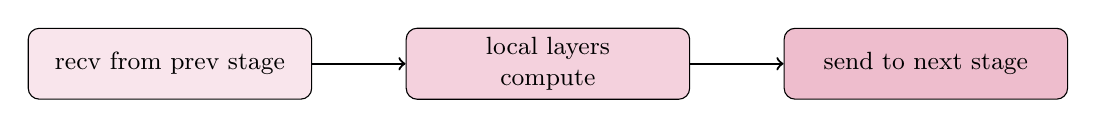
\begin{tikzpicture}[every node/.style={font=\small, align=center}]
\node[draw, rounded corners, fill=purple!10, minimum width=3.6cm, minimum height=0.9cm] (recv) at (0,0) {recv from prev stage};
\node[draw, rounded corners, fill=purple!18, minimum width=3.6cm, minimum height=0.9cm] (comp) at (4.8,0) {local layers\\compute};
\node[draw, rounded corners, fill=purple!26, minimum width=3.6cm, minimum height=0.9cm] (send) at (9.6,0) {send to next stage};
\draw[->, thick] (recv) -- (comp);
\draw[->, thick] (comp) -- (send);
\end{tikzpicture}
\caption{流水线并行的 rank 内循环：先接收，再计算，再发送}
\end{figure}

\begin{warningbox}{流水线并行的常见问题}
\begin{itemize}
    \item stage 负载不均会让最慢的 stage 决定整体速度。
    \item microbatch 太少，bubble 很大。
    \item 计算和通信若不能 overlap，效率会明显掉下来。
\end{itemize}
\end{warningbox}

\begin{lstlisting}[caption={流水线并行的极简理解},label={lst:pp}]
for microbatch in chunks(batch):
    if rank > 0:
        recv(x)
    for W in local_layers:
        x = gelu(x @ W)
    if rank + 1 < world_size:
        send(x)
\end{lstlisting}

\begin{knowledgebox}{流水线并行的核心}
它把“深模型的一串层”拆成几个 stage，然后让激活像传送带一样往前走。难点不在层本身，而在怎么把 stage 排得尽量均衡。
\end{knowledgebox}

\subsection{流水线效率的近似公式}

流水线并行不是“把层切开”就自动高效。它的效率常常可以用一个非常粗的近似来理解：
\[
\eta_{\text{pipe}} \approx \frac{M}{M + S - 1},
\]
其中 $M$ 是 microbatch 数，$S$ 是 stage 数。这个式子直接告诉你：\textbf{stage 越多，空档越大；microbatch 越少，利用率越低。}

\begin{table}[H]
\centering
\small
\begin{tabular}{p{2.3cm}p{2.5cm}p{3.6cm}p{4cm}}
\toprule
\textbf{stage 数 $S$} & \textbf{microbatch 数 $M$} & \textbf{近似效率} & \textbf{直觉} \\
\midrule
4 & 4 & $4/7 \approx 57\%$ & 空档明显 \\
4 & 8 & $8/11 \approx 73\%$ & 已开始像流水线 \\
4 & 16 & $16/19 \approx 84\%$ & 利用率较高 \\
8 & 8 & $8/15 \approx 53\%$ & stage 多时更容易浪费 \\
\bottomrule
\end{tabular}
\caption{microbatch 数与流水线效率的关系}
\end{table}

\begin{warningbox}{microbatch 不是越碎越好}
microbatch 越多，pipeline bubble 越小，但调度、通信和 kernel launch 次数都会上升。实际训练里要在”利用率”和”额外开销”之间找平衡。
\end{warningbox}

\subsection{Worked Example：流水线 bubble 开销的精确计算}

用一组具体数字来感受 bubble 的代价。假设每个 microbatch 通过一个 stage 的计算时间为 $t_f$（前向）和 $t_b$（反向），且 $t_b \approx 2 t_f$（反向通常比前向慢 $\sim$2 倍）。

\begin{table}[H]
\centering
\small
\begin{tabular}{p{3.8cm}p{2.5cm}p{2.5cm}p{3.5cm}}
\toprule
\textbf{配置} & \textbf{bubble 时间} & \textbf{有效计算时间} & \textbf{bubble 占比} \\
\midrule
$S=4$, $M=4$, $t_f=10$ms & $(S-1) \cdot t_f = 30$ms & $M \cdot (t_f + t_b) = 120$ms & $30/150 = 20\%$ \\
$S=4$, $M=8$ & $30$ms & $240$ms & $30/270 = 11\%$ \\
$S=4$, $M=16$ & $30$ms & $480$ms & $30/510 = 5.9\%$ \\
$S=4$, $M=32$ & $30$ms & $960$ms & $30/990 = 3.0\%$ \\
$S=8$, $M=8$ & $70$ms & $240$ms & $70/310 = 22.6\%$ \\
$S=8$, $M=32$ & $70$ms & $960$ms & $70/1030 = 6.8\%$ \\
\bottomrule
\end{tabular}
\caption{不同 stage 数和 microbatch 数下的 bubble 开销。$t_f = 10$ ms, $t_b = 20$ ms。}
\end{table}

更一般的 bubble 占比公式为：
$$
\text{bubble ratio} = \frac{(S - 1) \cdot t_f}{M \cdot (t_f + t_b) + (S-1) \cdot t_f} \approx \frac{S-1}{3M + S - 1}
$$
其中假设 $t_b \approx 2t_f$。要把 bubble 控制在 5\% 以内，需要 $M \geq \frac{19(S-1)}{3}$。对 $S=4$，这意味着 $M \geq 19$；对 $S=8$，需要 $M \geq 44$。

\begin{warningbox}{流水线并行的 Bubble 问题与 1F1B 调度}
上面的分析假设的是最朴素的 GPipe 调度——先做完所有 microbatch 的前向，再做所有 microbatch 的反向。这种调度有两个问题：
\begin{enumerate}
    \item \textbf{Bubble 大}：fill 和 drain 阶段都有空闲 stage。
    \item \textbf{激活内存高}：所有 microbatch 的中间激活必须同时保留，直到反向计算。
\end{enumerate}

\textbf{1F1B}（One Forward One Backward）调度通过交替执行前向和反向来缓解这两个问题：
\begin{itemize}
    \item 在 steady state 阶段，每个 stage 交替做一次前向、一次反向。
    \item 激活内存从 $O(M)$ 降低到 $O(S)$——每个 stage 只需保留 $S$ 个 microbatch 的激活。
    \item Bubble 比例与 GPipe 相同（$\frac{S-1}{M+S-1}$），但内存效率大幅提升。
\end{itemize}
更进一步的调度如 \textbf{interleaved 1F1B}（Megatron-LM 使用）可以把 bubble 再减半，代价是每个 rank 需要持有多段不连续的层。
\end{warningbox}

\begin{figure}[H]
\centering
\begin{tikzpicture}[font=\small]
\draw[->] (0,0) -- (10.5,0) node[right]{time};
\draw[->] (0,0) -- (0,4.4) node[above]{stage};
\foreach \x/\c in {1/blue!12,2/blue!18,3/blue!24,4/blue!30,5/blue!36,6/blue!42}{
    \draw[fill=\c] (\x,0.5) rectangle ++(0.7,0.55);
    \draw[fill=\c] (\x+1,1.35) rectangle ++(0.7,0.55);
    \draw[fill=\c] (\x+2,2.2) rectangle ++(0.7,0.55);
    \draw[fill=\c] (\x+3,3.05) rectangle ++(0.7,0.55);
}
\node[anchor=west] at (7.9,3.9) {中间阶段最忙};
\node[anchor=west] at (7.9,3.5) {首尾阶段有灌入/排空空档};
\end{tikzpicture}
\caption{流水线调度的典型形态：不是每个 stage 都能同时满负载}
\end{figure}

\subsection{stage 负载不均会怎样}

如果某个 stage 远重于其他 stage，那么整条 pipeline 都会被拖慢。换句话说，流水线的吞吐量大致由最慢的 stage 决定，而不是由平均 stage 决定。这也是为什么切 stage 时不能只按层数平均，还要看每层到底有多少计算量。

\begin{importantbox}{流水线切分的核心准则}
切 stage 时，不是“每个 rank 分到一样多的层”就够了，而是要尽量让每个 stage 的计算时间接近。否则瓶颈 stage 会把整条流水线的效率压低。
\end{importantbox}

\begin{figure}[H]
\centering
\begin{tikzpicture}[every node/.style={font=\small, align=center}]
\node[draw, rounded corners, fill=green!12, minimum width=2.6cm, minimum height=0.9cm] (a) at (0,0) {stage 0\\轻};
\node[draw, rounded corners, fill=green!24, minimum width=3.5cm, minimum height=0.9cm] (b) at (4.0,0) {stage 1\\重};
\node[draw, rounded corners, fill=green!12, minimum width=2.6cm, minimum height=0.9cm] (c) at (8.6,0) {stage 2\\轻};
\node[draw, rounded corners, fill=green!12, minimum width=2.6cm, minimum height=0.9cm] (d) at (12.0,0) {stage 3\\轻};
\draw[->, thick] (a) -- (b);
\draw[->, thick] (b) -- (c);
\draw[->, thick] (c) -- (d);
\end{tikzpicture}
\caption{stage 不均衡会把吞吐量拉到最重的那一段上}
\end{figure}

